\chapter{Многомодовые когерентные состояния и их интерференция}  \label{ch:ch4}

\section{Классическое описание многомодовых когерентных состояний} \label{sec:ch4/sec1}

Покажем, как в системах квантовой коммуникации на боковых частотах формируются многомодовые когерентные состояния в результате фазовой модуляции с точки зрения волновой оптики. Аналитически работа модуляторов описывается следующим образом. Пусть несущая оптическая частота задана выражением $Ae^{i \omega t}$ (A - амплитуда, $\omega$ - частота несущей). После модуляции в блоке отправителя (Алисы) при индексе модуляции $m$, используя разложение Якоби-Ангера, получаем сигнал: 

\begin{equation}
	\begin{aligned}
	\label{eq:equation4_1}
		E = Ae^{i \omega t}e^{i \alpha sin(\Omega t+ \varphi_a)} = Ae^{i \omega t} \sum_{n=-\infty}^\infty J_{n}(m) e^{i (\Omega t+ \varphi_a) n},
	\end{aligned}
\end{equation}

где  $\Omega$ - частота модулирующего сигнала, $m$ - индекс модуляции, $\varphi_a$ - фаза модулирующего сигнала, вводимая на стороне отправителя, $J_{n}(m)$ - функция Бесселя первого рода, $n$ - номер моды. Из выражения (\ref{eq:equation4_1}) видно, что в результате модуляции вдобавок к основной частоте $\omega$ в спектре появляются сигналы на боковых частотах  $\omega + n$  и  $\omega - n$ по обе стороны от центральной частоты, как показано на рисунке \ref{fig:multimodes_clas}. 

\begin{figure}[ht]
  \centering
  \includegraphics[scale=0.6]{Modes_rus_clas.pdf}
  \caption{Принципиальная схема формирования боковых (поднесущих) частот}
  \label{fig:multimodes_clas}
\end{figure}

%%%%%%%%%%%%%%%%%%%%%%%%%%%%%%%%%%%%%%%%%%%%%%%%%%%%%%%%%%%%%%%%%%%%%%%%%%%%%%%%%%%%%%%%%%%%%%%%%%%%%%%%%%%%%%%%%
\section{Исследование зависимости результата интерференции многомодовых состояний от разности фаз модулирующих сигналов в классическом приближении} \label{sec:ch4/sec2}

Обычно измерительной оборудование (ДОФ) находится на стороне приёмного модуля. В случае вынесения измерительного оборудования в недоверенный узел, требуется формировать сигналы, а также модулировать их независимо Алисой (a) и Бобом (b). Соответствующие сигналы имеют следующий вид:

\begin{equation}
	\begin{aligned}
	\label{eq:equation4_2_1}
		E_a = Ae^{i \omega t} \sum_{n=-\infty}^\infty J_{n}(m) e^{i (\Omega t+ \varphi_a) n},
	\end{aligned}
\end{equation}

\begin{equation}
	\begin{aligned}
	\label{eq:equation4_2_2}
		E_b = Ae^{i \omega t} \sum_{n=-\infty}^\infty J_{n}(m) e^{i (\Omega t+ \varphi_b) n},
	\end{aligned}
\end{equation}

Выражения (\ref{eq:equation4_2_1}) и (\ref{eq:equation4_2_2}) можно преобразовать к виду, где явно вынесена компонента, зависящая от фазы модулирующего сигнала $\varphi_a$ и $\varphi_b$ :

\begin{equation}
	\begin{aligned}
	\label{eq:equation4_2_3}
		E_a = \sum_{n=-\infty}^\infty A J_{n}(m) e^{i t (\omega + \Omega n)} e^{i \varphi_a n},
	\end{aligned}
\end{equation}

\begin{equation}
	\begin{aligned}
	\label{eq:equation4_2_4}
		E_b = \sum_{n=-\infty}^\infty A J_{n}(m) e^{i t (\omega + \Omega n)} e^{i \varphi_b n},
	\end{aligned}
\end{equation}


Интерференция когерентных многомодовых состояний, приходящих от легитимных пользователей, происходит на светоделителе, выходы которого подключены к измерителям оптической мощности. Из-за разности оптических путей между несущими частотами будет также наблюдаться разность фаз $\varphi_0$, влияющая на картину интерференции. Амплитуда сигналов (\ref{eq:equation4_2_3}) и (\ref{eq:equation4_2_4}) поступающих на измерители, приобретает следующий вид в результате интерференции:

\begin{equation}
	\begin{aligned}
	\label{eq:equation4_2_5}
		E_{ab} = \sum_{n=-\infty}^\infty \frac{A J_{n}(m) e^{i t (\omega + \Omega n)}}{\sqrt{2}} (e^{i \varphi_a n} \pm e^{i \varphi_b n}e^{i \varphi_0}),
	\end{aligned}
\end{equation}

Наблюдается зависимость от фаз, вносимых Алисой и Бобом, для членов ряда. Измерительные приборы фиксируют модуль квадрата амплитуды входящих когерентных многомодовых состояний после вырезания спектральным фильтром нулевой моды, так что в зависимости от разности фаз $\Delta \phi = \varphi_b-\varphi_a$ и, с учетом потерь в квантовом канале и квантовой эффективности $\eta_c$ измерителей оптического сигнала, мы получим:

\begin{equation}
	\begin{aligned}
	\label{eq:pdetclas}
 		P(\Delta\varphi)&=\eta_c |A|^2 \Big(1-(1\mp\cos(\varphi_0)) J_{0}(m)^2 \pm \cos(\varphi_0) J_{0}(m\sqrt{2(1+\cos(\Delta\phi))}) \Big),
	\end{aligned}
\end{equation} 

Определим величину среднее число фотонов на многомодовых когерентных состояниях в отсутствие нулевой моды $\mu$ следующим образом: 

\begin{equation}
	\begin{aligned}
	\label{eq:muclas}
		\mu = |A|^2 (1-J_{0}(m)^2)	
	\end{aligned}
\end{equation}

Так как значение нулевой моды функции Бесселя равно:

\begin{equation}
	\begin{aligned}
	\label{eq:carrclas}
		J_{0}(m)^2 = 1-\frac{m^2}{2} 	
	\end{aligned}
\end{equation}

то при индексе модуляции $m < 1$  выражение (\ref{eq:equation4_2_5}) принимает вид:

\begin{equation}
	\begin{aligned}
	\label{eq:mulow}
		\mu = |A|^2 \frac{m^2}{2}
	\end{aligned}
\end{equation}


Используя (\ref{eq:muclas}), (\ref{eq:carrclas}) и (\ref{eq:mulow}), выражение (\ref{eq:pdetclas}) для мощностей, наблюдаемых на выходах светоделителя в результате интерференции многомодовых состояний, приходим к следующему выражению: 

\begin{equation}
	\begin{aligned} 
	\label{eq:pinterf}
 		P(\Delta\varphi)&=\mu\eta_c(1\pm\cos(\Delta\varphi)\cos(\varphi_0)),
	\end{aligned}
\end{equation}

Наблюдается зависимость интенсивности многомодовых когерентных состояний от разности фаз $\Delta\phi$ модулирующих сигналов и от фазы $\phi_0$ оптического сигнала несущей частоты Алисы относительно несущей частоты Боба.

%%%%%%%%%%%%%%%%%%%%%%%%%%%%%%%%%%%%%%%%%%%%%%%%%%%%%%%%%%%%%%%%%%%%%%%%%%%%%%%%%%%%%%%%%%%%%%%%%%%%%%%%%%%%%%%%%
\section{Квантовое описание когерентного состояния} \label{sec:ch4/sec3}
Термин \textit{когерентное состояние} был введен Р. Дж. Глаубером. в 1963 г. Оно не совсем соотносится с классическим термином когерентность, но имеет отношение к специальному типу чистых квантово-механических состояний светового поля, соответствующего одиночной моде резонатора. Когерентное состояние определяется, как суперпозиция Фоковских состояний, то есть состояний числа фотонов. 


\begin{equation}
	\begin{aligned}
		|\alpha \rangle = \sum_{n=0}^\infty   |  \rangle,
	\end{aligned}
\end{equation}

Комплексное число $ \alpha $	определяется среднее число фотонов, которое равно квадрату модуля, и фазой когерентного состояния. Из выражения видно, что вероятность нахождения n фотонов в когерентном состоянии определяется, как показано в уравнении. 

\begin{equation}
	\begin{aligned}
		|\alpha \rangle = \sum_{n=0}^\infty   |  \rangle,
	\end{aligned}
\end{equation}

где - это среднее число фотонов. Видно, что когерентное состояние подчиняется распределению Пуассона. Когерентное состояние имеет свойства близкие классическим состояниям света. Отдельный случай когерентного состояния - это когда n=0. Оно называется вакуумным состоянием с нулевым числом фотонов. Однако, в таком случае все равно наблюдаются квантовые флуктуации электрического и магнитного полей, которые иногда называют вакуумным шумом. 


%	\pagebreak

%%%%%%%%%%%%%%%%%%%%%%%%%%%%%%%%%%%%%%%%%%%%%%%%%%%%%%%%%%%%%%%%%%%%%%%%%%%%%%%%%%%%%%%%%%%%%%%%%%%%%%%%%%%%%%%%%
\section{Когерентные состояния после прохождения светоделителя} \label{ch:ch4/sec4}
 
Рассмотрим следующую систему: на вход светоделителя 2х2 подается когерентное состояние $| \psi \rangle_{\alpha}$, формируемое лазерным источником Л1. На второй порт поступает вакуумное состояние $| \psi \rangle_{\beta}$. При этом:

\begin{equation}
	| \psi \rangle_{\alpha} = | \alpha_{0} e^{i\phi_{0}k} \rangle \\
\end{equation}

\begin{equation}
	| \psi \rangle_{\beta} = | vac \rangle \\
\end{equation}


На обоих выходах светоделителя будет состояние  $| \frac{\alpha_{0}}{\sqrt{2}} \rangle$, поступающее на электро-оптические фазовые модуляторы ФМ1 и ФМ2. В результате фазовой модуляции состояние преобразуется в $| \alpha_{1} \rangle$ и $| \alpha_{2} \rangle$. 


 \begin{figure}[ht]
  \centering
  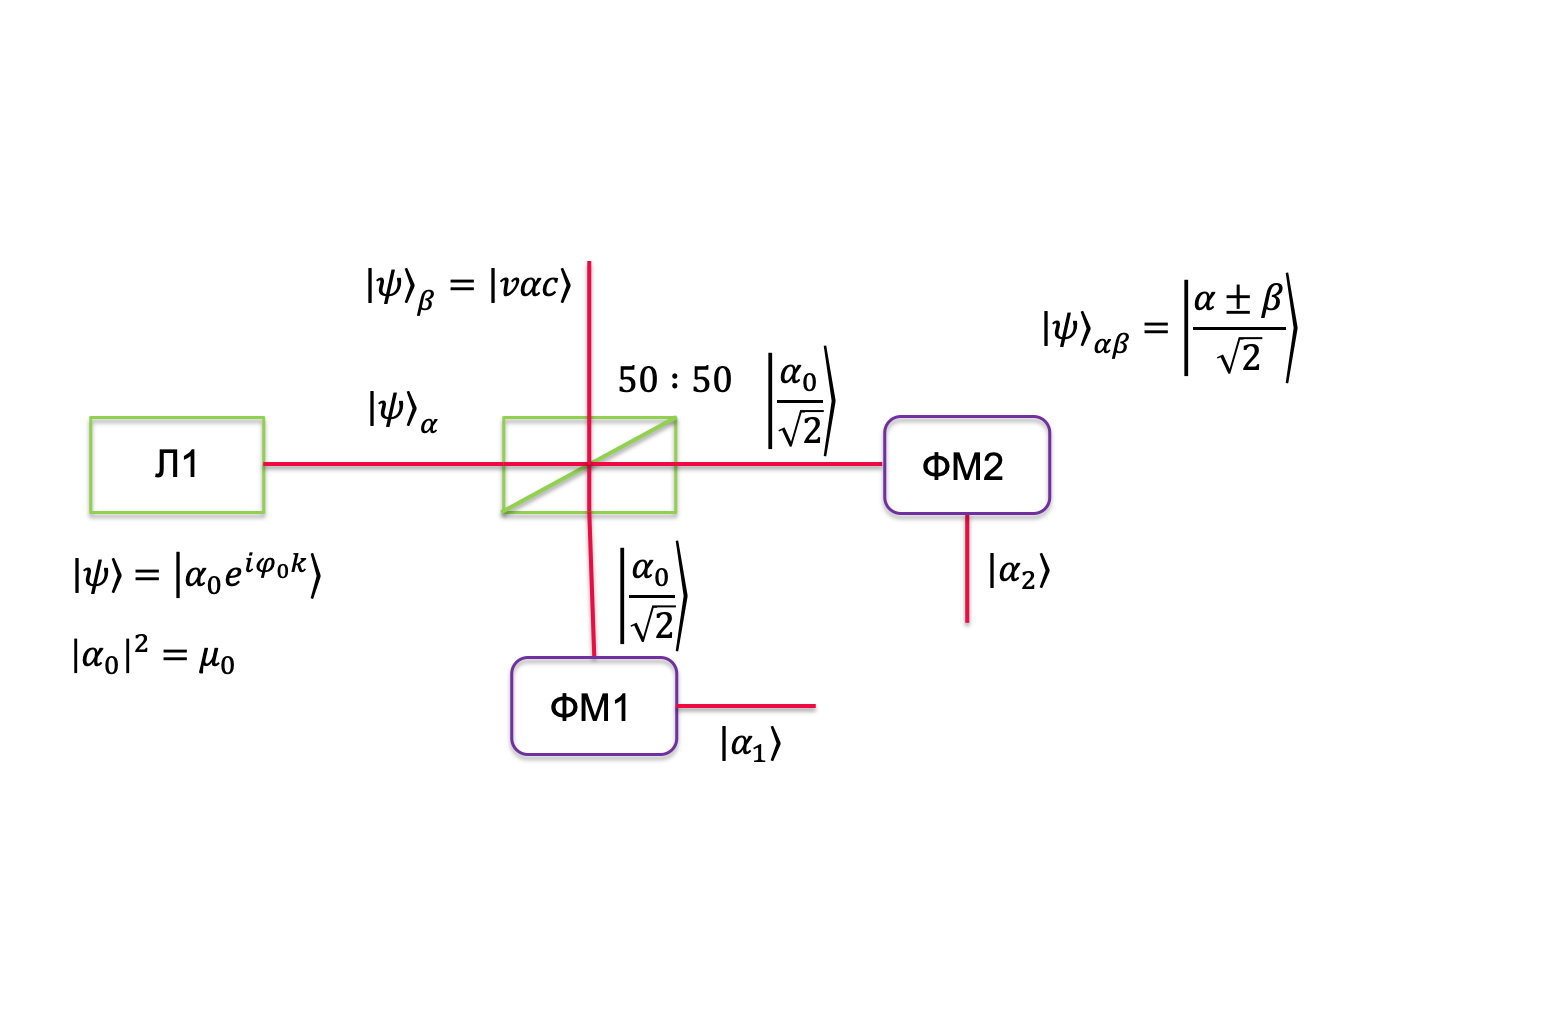
\includegraphics[scale=0.6]{Coherent_states_beamsplitting.png}
  \caption{Принципиальная схема наблюдения динамики когерентных состояний}
  \label{fig:Coherent_states_beamsplitting}
\end{figure}

\pagebreak

%%%%%%%%%%%%%%%%%%%%%%%%%%%%%%%%%%%%%%%%%%%%%%%%%%%%%%%%%%%%%%%%%%%%%%%%%%%%%%%%%%%%%%%%%%%%%%%%%%%%%%%%%%%%%%%%%
\section{Когерентные состояния после модуляции} \label{ch:ch4/sec5}

Отличительно особенностью систем квантовой коммуникации на боковых частотах модулированного излучения является генерация многомодовых когерентных состояний на разных оптических модах, зависящих от частоты модулирующего сигнала, как показано на рисунке \ref{fig:multimodes_q}. 

 \begin{figure}[ht]
  \centering
  \includegraphics[scale=0.6]{Modes_rus.pdf}
  \caption{Принципиальная схема генерации боковых частот}
  \label{fig:multimodes_q}
\end{figure}


Определим приготовленные состояния. Входное (немодулированное) состояние на стороне модулятора отправителя (Алиса) и получателя (Боб) (далее именуемые, как $A$ or $B$) определяется, как $|\sqrt{\mu_0}\rangle_0\otimes|\mathrm{vac}\rangle_{SB}$, где $|\mathrm{vac}\rangle_{SB}$ это вакуумное состояние на боковых и $|\sqrt{\mu_0}\rangle_0$ это когерентное состояние несущей частоты с амплитудой, определенной средним числом фотонов $\mu_0$ в окне пропускания. формируемая когерентным монохроматическим излучением с оптической частотой $\omega$. Фаза несущей волны принимается как опорная и все остальные фазы считаются по отношению к ней. Электро-оптический фазовый модулятор (с частотой колебаний микроволнового поля $\Omega$ и её фазой $\varphi_A$ или $\varphi_B$) перераспределяет энергию между взаимодействующими модами (поле на выходе модулятора приобретает боковые частоты $\omega_k=\omega+k\Omega$, ограничим рассматриваемый нами случай $2S$ боковыми частотами и пусть целое число $k$ мод ограничено пределами $-S\le k\le S$), так, что состояние поля на выходе модулятора - это многомодовое когерентное состояние: 
%
\begin{equation}\label{phi}
|\psi_0(\varphi_j)\rangle = \bigotimes_{k=-S}^S|{\alpha_k(\varphi_j)}\rangle_k,
\end{equation}
%
где $j$ это и $A$, и $B$ (определяющее Алису или Боба), а амплитуды имеют следующий вид: 
%
\begin{equation}\label{alpha}
\alpha_k(\varphi_j)=\sqrt{\mu_0}d^S_{0k}(\beta)e^{i\varphi_jk},
\end{equation}
%
и $d^S_{nk}(\beta)$ это d-функция Вигнера, взятая из квантовой теории углового момента \cite{varshalovich1988quantum}, $\beta$ определяется индексом модуляции $m$, который без учета дисперсии в среде модулятора можно выразить: 
%
\begin{equation}\label{betam}
\cos{({\beta})}=1-\frac{1}{2}{\left(\frac{m}{S+0.5}\right)^2},
\end{equation}
где $S$ количество взаимодействующий мод, принимаемое очень большим. 

\pagebreak

%%%%%%%%%%%%%%%%%%%%%%%%%%%%%%%%%%%%%%%%%%%%%%%%%%%%%%%%%%%%%%%%%%%%%%%%%%%%%%%%%%%%%%%%%%%%%%%%%%%%%%%%%%%%%%%%%
\section{Результат интерференции когерентных состояний после модуляции} \label{ch:ch4/sec6}

После распространения по квантовому каналу амплитуда когерентного состояния ослабляется и имеет следующий вид:

\begin{equation}
\sqrt{\eta_c}\alpha_k(\varphi_j)=\sqrt{\mu_0\eta_c}d^S_{0k}(\beta)e^{i\varphi_jk},
\end{equation}


где $\eta_c$ оптическое пропускание канала. На втором светоделителе состояния преобразуются в следующий вид: 

\begin{align}\label{states}
\Big|\frac{\alpha_A \pm \alpha_Be^{i\varphi_0}}{2}\Big\rangle_{1,2} &= \bigotimes_{k=-S}^{S}\Big|\sqrt{\frac{\mu_0\eta_c}{2}}d_{0k}^{S}(\beta)\left(e^{i\varphi_Ak}\pm e^{i(\varphi_Bk+\varphi_0)}\right)\Big\rangle_k.
\end{align}
Выражение с плюсом определяется, как состояние на первом выходе второго светоделителя (нижний индекс $1$), а выражение с минусом как состояние на втором выходе второго светоделителя (нижний индекс  $2$). 
 
\begin{figure}[ht]
 \centering
  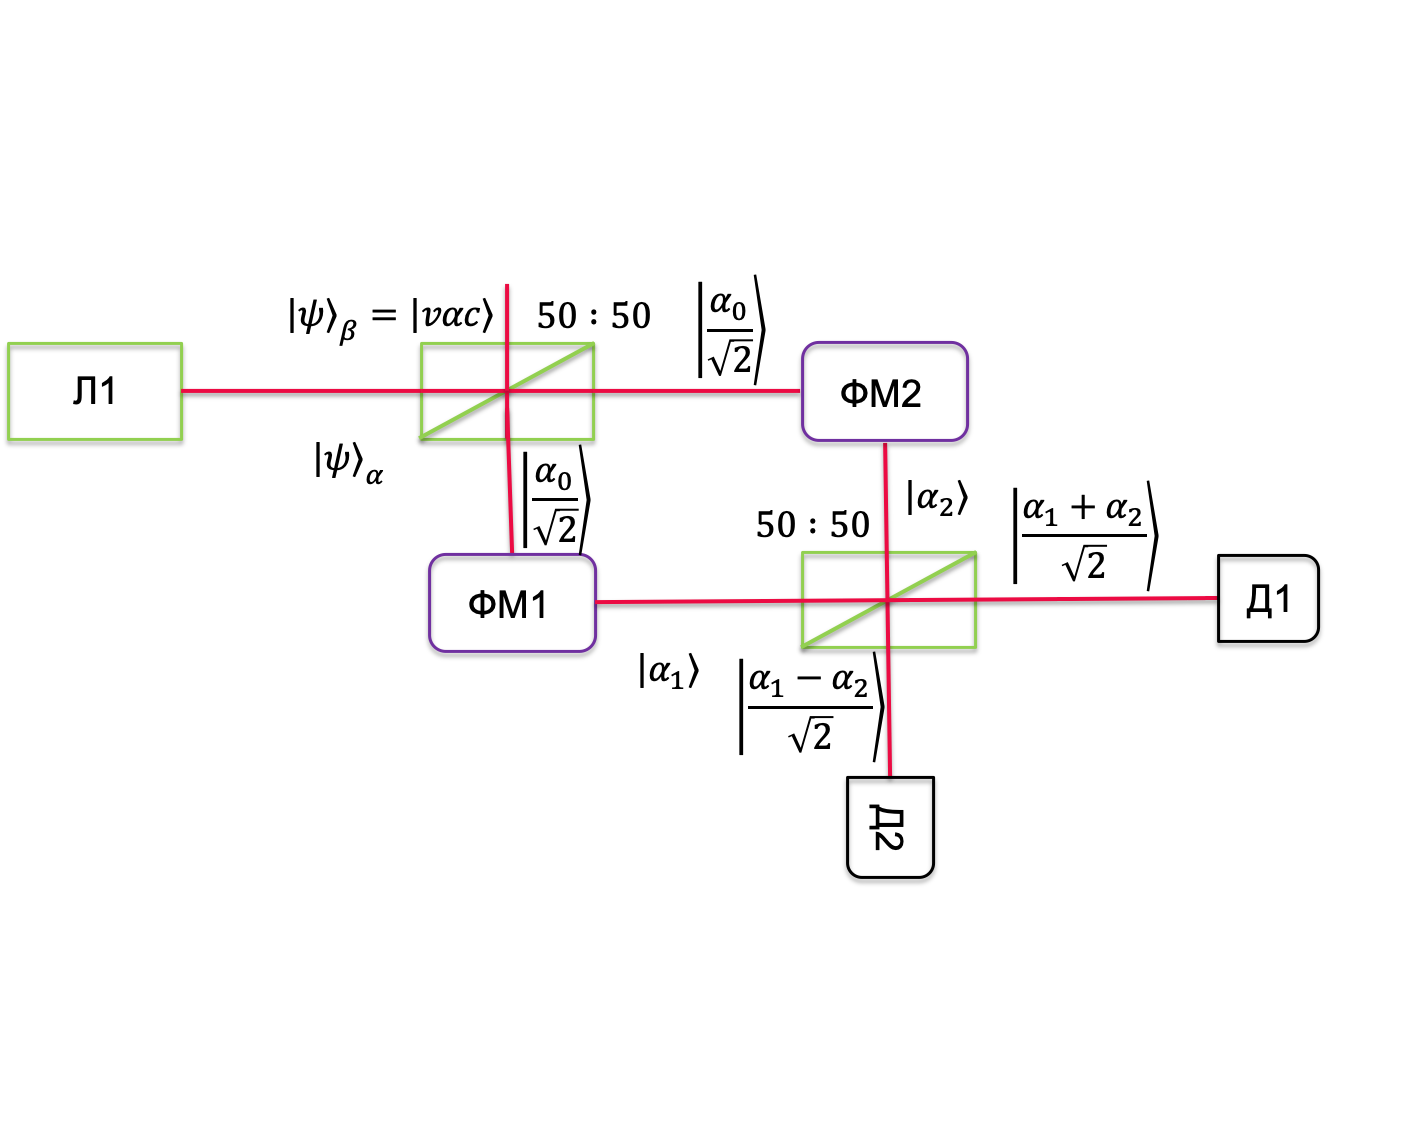
\includegraphics[scale=0.6]{Coherent_state_beamsplitting2.png}
  \caption{Принципиальная схема наблюдения динамики когерентных состояний}
  \label{fig:Coherent_states_beamsplitting2}
\end{figure}

\pagebreak

%%%%%%%%%%%%%%%%%%%%%%%%%%%%%%%%%%%%%%%%%%%%%%%%%%%%%%%%%%%%%%%%%%%%%%%%%%%%%%%%%%%%%%%%%%%%%%%%%%%%%%%%%%%%%%%%%
\section{Зависимость результата интерференции от разности фаз когерентных состояний} \label{ch:ch4/sec7}

После подстройки относительной фазы оптических сигналов в двух плечах, наблюдается интерференция этих состояний на втором светоделителе (СД2). Описание состояний на выходах светоделителя дано в уравнении (\ref{states}). Далее предполагается, что относительная фазовая отстройка оптических импульсов равна $\phi_0\approx0$. Если разность фаз между радиочастотными модулирующими сигналами Алисы и Боба равна нулю ($\Delta\varphi=0$) весь спектр идет в одно выходное плечо светоделителя СД2, в ином случае, четные моды спектра, включая центральную, идут в то же плечо, а нечетные идут во второе плечо. В случае $\Delta\varphi=0$, требуется спектральное разделение центральной частоты и боковых в приёмном блоке, так как кодирование квантовых состояний происходит на боковых частотах. Следует учитывать, что при использовании малого среднего числа фотонов в импульсе, значительный вклад в многомодовых состояниях вносят только первая пара боковых частот. Случай, при котором $\Delta\varphi=\pi$, является нетривиальным. Многомодовое состояние разделяется на СД2 и центральная мода (и все четные) идут в первое плечо, а все нечетные (первые боковые частоты вносят наибольший вклад в результирующий сигнал) идут во второе плечо, как показано на рисунке \ref{fig:Interference_result}. Таким образом, можно отказаться от спектрального разделения при помощи оптического фильтра в одном из выходных плечей приёмного узла. Показателем хорошей подстройки по фазе оптических импульсов является постоянный высокий уровень на центральной частоте в первом плече (на Д2).  


\begin{figure}[ht]
 \centering
  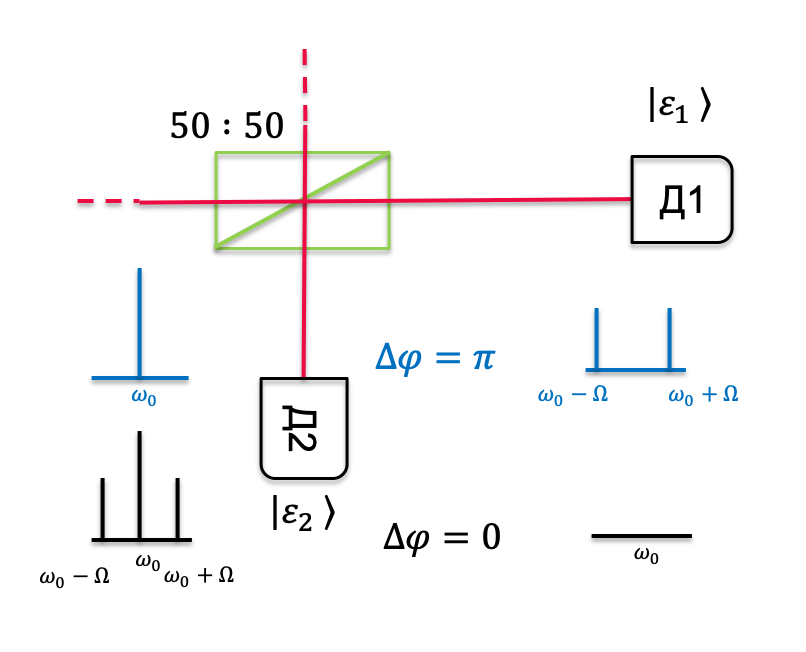
\includegraphics[scale=0.9]{Interference_result.png}
  \caption{Принципиальная схема наблюдения результата интерференции когерентных состояний}
  \label{fig:Interference_result}
\end{figure}

\pagebreak

%%%%%%%%%%%%%%%%%%%%%%%%%%%%%%%%%%%%%%%%%%%%%%%%%%%%%%%%%%%%%%%%%%%%%%%%%%%%%%%%%%%%%%%%%%%%%%%%%%%%%%%%%%%%%%%%%
\section{Протокол системы квантовой рассылки ключа, устойчивый к атакам на измерительное оборудование} \label{ch:ch4/sec8}

Основываясь на полученных результатах можно сформулировать протокол для системы квантовой коммуникации, использующей многомодовые когерентные состояния, с недоверенным измерительным узлом (рис. \ref{fig:Protocol}). Для простоты приведем пример с использованием только двух фазовых состояний по аналогии с протоколом B92. Алиса случайным образом выбирает одно фазовое состояние из двух возможных <<$0$>> или <<$\pi$>>. Боб независимо от Алисы тоже случайным образом выбирает одно из двух фазовых состояний. В результате интерференции многомодовых когерентных состояний можно наблюдать 4 различных варианта, в зависимости от разности фаз, выбранных Алисой и Бобом.  При этом на недоверенном узле регистрации будет происходить спектральное разделение, описанное в разделе \ref{ch:ch4/sec7}, так что на Д1 и Д2 будут поступать боковые частоты. Злоумышленник при этом имеет полный доступ к недоверенному измерительному узлу и может фиксировать себе оглашенный результат срабатываний одного из детекторов. Положим, что нас интересует только случай, при котором разность фаз между А и Б равна $\pi$. Преимущество этого случая в том, что за счет спектрального разделения в результате интерференции в плечо с детектором Д1 всегда будут идти только боковые и никогда не будет идти центральная мода, а значит можно исключить из оптической схемы этого плеча оптический фильтр, согласование которого с фильтром в другом плече -- достаточно трудная инженерная задача. Таким образом, при просеивании остаются только те биты, которые соответствуют отсчетам на Д1, при этом для корреляции между битами Алисы и битами Боба последний должен сделать смену бита на противоположный (так называемый <<bitflip>>).  

\begin{figure}[ht]
 \centering
  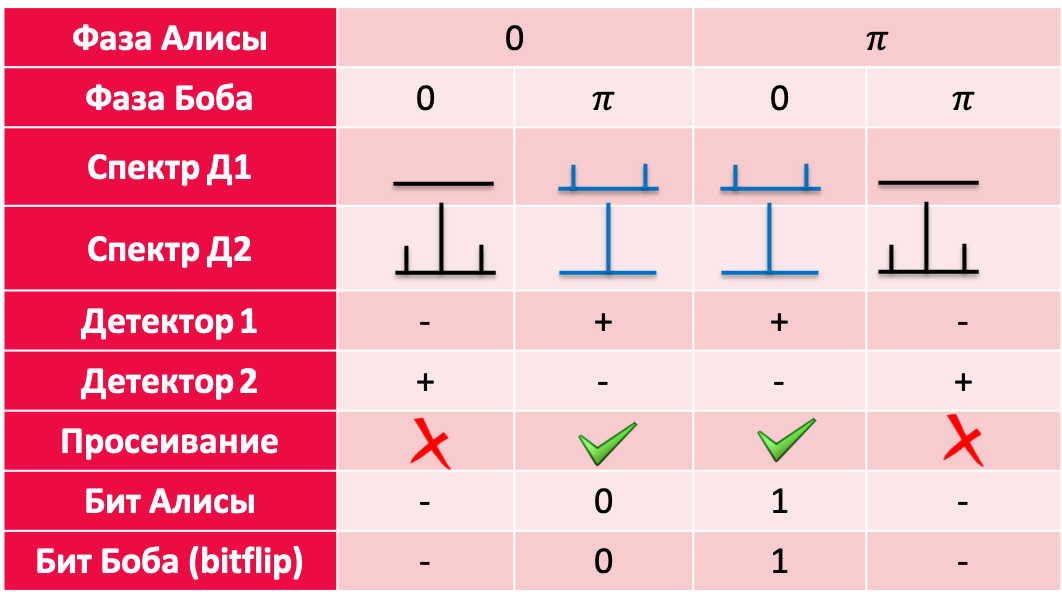
\includegraphics[scale=0.9]{Protocol.png}
  \caption{Протокол}
  \label{fig:Protocol}
\end{figure}


\pagebreak

%%%%%%%%%%%%%%%%%%%%%%%%%%%%%%%%%%%%%%%%%%%%%%%%%%%%%%%%%%%%%%%%%%%%%%%%%%%%%%%%%%%%%%%%%%%%%%%%%%%%%%%%%%%%%%%%%
\section{Выводы по главе} \label{ch:ch4/sec9}


В \ref{ch:ch4} главе показано, что метод квантовой коммуникации на боковых частотах позволяет реализовывать протокол, устойчивый к контролю нелегитимным пользователем измерительного оборудования. 
 
\pagebreak

